\section{Conclusion}

\subsection{Reflection}

For a direct marketing campaign, it is essential to correctly identify the customers who will respond to a particular campaign.

In this project, we analyzed demographic data for customers of a mail-order sales company in Germany, comparing it against demographics information for the general population. Exploratory Data Analysis was performed to understand and clean the data. Unsupervised learning techniques were used to perform customer segmentation, identifying the parts of the population that best describe the core customer base of the company. Then, we applied what we've learned on a third dataset with demographic information for targets of a marketing campaign for the company, and use a model to predict which individuals are most likely to convert into becoming customers for the company (all of this is reflected in Figure \ref{fig:final_pipeline}).

This project was an excellent opportunity to apply and learn new techniques primarily related to imbalanced data problems. Also going beyond simple grid search for hyper-parameter tuning was both a new tool to learn and also a time saver.

\begin{figure}[h]
\centering
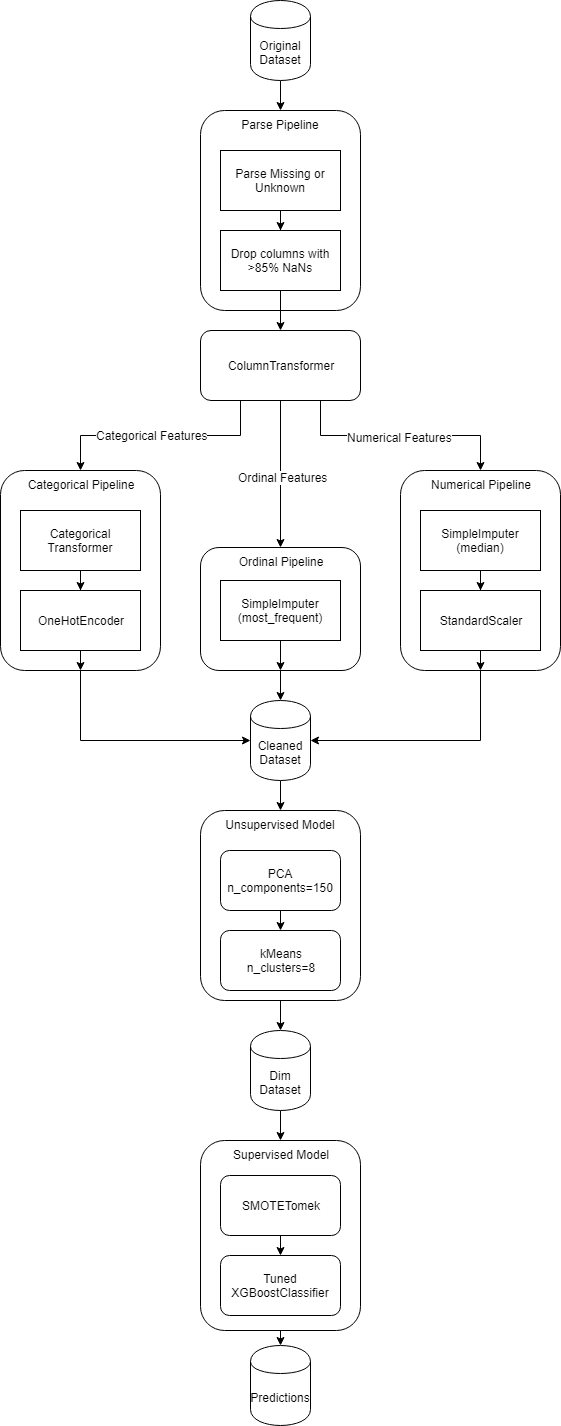
\includegraphics[width=0.5\textwidth, height=0.8\textwidth]{images/final_pipeline.png}
\caption{Entire project pipeline}
\label{fig:final_pipeline}
\end{figure}

\subsection{Improvement}

Reflecting on the steps taken in this project, we can identify some areas where improvements can be made:
\begin{itemize}
    \item Data preprocessing - Engineer more categorical features: We believe that better results can be obtained if more categorical features are treated like mixed-type features and re-engineered.
    \item Data preprocessing - Missing Data: 
        \begin{itemize}
            \item Analyze if there is data missing at random or there are patterns. 
            \item Try to find correlations between missing values and use PCA to remove some of them
            \item Use a supervised model to predict the values for NaN instead of just filling with the median or mode.
        \end{itemize}
    \item Dimensionality Reduction - Use FAMD (Factor Analysis of Mixed Data) instead of applying PCA on both numerical and Categorical features
\end{itemize}